\documentclass{beamer}

\usepackage{german}	%Block zum Setzen von Umlauten
\usepackage{lmodern}
\usepackage[utf8]{inputenc}

\mode<presentation>
\definecolor{hdaRot}{cmyk}{0,1,1,0.18}     % -5005
\definecolor{hdaBlauMed}{cmyk}{0.71,0.25,0,0}     % -1169
\definecolor{hdaGruenMed}{cmyk}{0.5,0.13,1,0.06}    % -2048

\setbeamercolor*{kred}{fg=hdaRot}
\setbeamercolor*{kblue}{fg=hdaBlauMed}
\setbeamercolor*{kgreen}{fg=hdaGruenMed}
\setbeamercolor*{kblack}{fg=black}
\setbeamerfont{block body alerted}{size=\huge}
\setbeamerfont{block title alerted}{size=\huge}
\setbeamercovered{transparent=25}
\usebeamercolor{normal text}
\mode<all>

\newcommand{\hlblue}{%
 \usebeamercolor[fg]{normal text}%
 \only{\usebeamercolor[fg]{kblue}}}

\newcommand{\hlgreen}{%
 \usebeamercolor[fg]{normal text}%
 \only{\usebeamercolor[fg]{kgreen}}}

\newcommand{\hlblack}{%
 \usebeamercolor[fg]{normal text}%
 \only{\usebeamercolor[fg]{kblack}}}

\newcommand{\hlred}{%
 \usebeamercolor[fg]{normal text}%
 \only{\usebeamercolor[fg]{kred}}}

\usepackage{tikz}

\usetikzlibrary{arrows,decorations.pathmorphing,backgrounds,positioning,fit,petri}%

\makeatletter
\tikzset{pics/named scope code/.style={code={\tikz@fig@mustbenamed%
  \begin{scope}[local bounding box/.expanded=\tikz@fig@name]#1\end{scope}%
}}}
\makeatother


\tikzset {
  pics/p2way/.style n args = {2}{
    named scope code = {
      \draw[line width=1pt]  (0,0) circle (1cm);
      \foreach \angle in {0, 180}{ \draw[line width=1pt] (\angle:0cm) -- (\angle:1cm); }
      \foreach \angle / \label in {90/#1, 270/#2}{ \draw (\angle:0.6cm) node{\textbf{\label}}; }
    }
  }
}

\begin{document}
\begin{frame}[t,shrink=65]
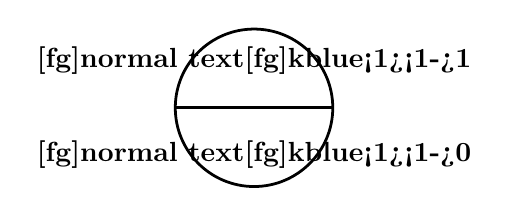
\begin{tikzpicture}
   [bend angle=45,
   line width=1pt,
   auto,
   pre/.style={<-,shorten <=1pt,>=stealth',semithick},
   post/.style={->,shorten >=1pt,>=stealth',semithick}]

   \pic (N01) at (0,4) {p2way=%
      {\hlblue<1>\visible<1->1}
      {\hlblue<1>\visible<1->0}
   };
  
 \end{tikzpicture}



\begin{columns}
\column[t]{.60\textwidth}

{\Large

\par\vspace{2cm}\noindent       %Abstand zur Grafik 2cm

    \begin{tabular}{l|lccl}
      \hline
      Nr & Tätigkeit        & Vorgänger & Aufwand & Kurz \\
      1  & Requirements     & -     & 2 & RQ \\
      2  & Studie           & -     & 1 & Studie \\
      3  & Systementwurf    & 1     & 4 & SE \\
      4  &   3              & 2     & - & \\
      5  & HW-Entwurf       & 3     & 3 & HW \\
      6  & Funktionsmuster  & 3     & 2 & FM \\
      7  & SW-Entwurf       & 3     & 3 & SW \\
      8  & Programmierung   & 7     & 6 & Pgm \\
      9  & 8                & 6     & - & \\
      10 & SW-Test          & 8     & 5 & SW-Test \\
      11 & Prototyp-Entwicklung & 5 & 5 & Proto \\
      12 & 11               & 6     & - & \\
      13 & HW-Test          & 11    & 4 & HW-Test \\
      14 & Integration      & 10; 13 & 2 & Int \\
      15 & System-Test      & 14    & 3 & Test \\
      \hline
        & \textbf{Gesamtaufwand} &   & \textbf{40} \\
    \end{tabular}
}

\column[t]{.40\textwidth}
\par\vspace{1cm}\noindent %Abstand
\begin{itemize}

{\huge
    \item<only@+> {Dein Netzplan beginnt immer bei einem FA(Frühester Anfang) von 0. Schreibe dies in die linke Spalte.}

    \item<only@+> {Suche alle Vorgänge ohne Vorgänger (siehe Liste). Alle diese Pfeile gehen von unserem ersten Knoten aus. Schreibe die Tätigkeiten (in Kurzform), sowie Aufwand/Dauer auf den Pfeil.}
    \item<only@+> {Schreibe den neuen FA in die linke Spalte. Hierbei addierst du den alten FA mit der Dauer T;
                   FA = FA + T}
    \item<only@+> {Füge alle Pfeile zu den möglichen Nachfolger hinzu. Vergiss die Beschreibung und Dauer nicht.}
    \item<only@+> {Ergänze FA.}
    \item<only@+> {Suche alle Knoten, die den jetzigen Knoten als Vorgänger haben.}
    \item<only@+> {Ergänze FA.}
    \item<only@+> {Schritt wie gewohnt.}
    \item<only@+> {Schritt wie gewohnt.}
    \item<only@+> {Bei einem Vorgang mit 2 oder mehr Vorgängern wie hier, wähle den mit dem höheren FA.}
    \item<only@+> {Schritt wie gewohnt.}
    \item<only@+> {Schritt wie gewohnt.}
    \item<only@+> {Übernehme den FA als SA(Spätester Anfang).}
    \item<only@+> {Die Differenz aus FA-SA ergibt die Pufferzeit.}
    \item<only@+> {Der neue SA wird aus der Differenz von SA und der Dauer eines Vorgangs berechnet . Pufferzeit wie gewohnt ausrechnen.}
    \item<only@+> {Schritt wie gewohnt.}
    \item<only@+> {Schritt wie gewohnt.}
    \item<only@+> {Schritt wie gewohnt.}
    \item<only@+> {Schritt wie gewohnt.}
    \item<only@+> {Hier wird der kleinste SA genommen.}
    \item<only@+> {Schritt wie gewohnt.}
    \item<only@+> {Schritt wie gewohnt.}
    \item<only@+> {Zeichne den kritischen Pfad ein (hier: rot markiert).}
    \item \alert<+> {}
}

\end{itemize}

\par\vspace{2cm}\noindent %Abstand

\only<1>{\begin{alertblock}{Merke!}
    Die Nummerierungen der Kreise haben nichts mit der Nummerierung der Vorgänge zu tun. Kreisnummer wird beliebig eingesetzt.
\end{alertblock}
}

\only<23>{\begin{alertblock}{Merke!}
   Alle Vorgänge mit einer Pufferzeit von 0 gehören zu dem kritischen Pfad.
\end{alertblock}
}

\end{columns}

\end{frame}

\end{document} 